\documentclass[14pt, conference, onecolumn]{IEEEtran}
\IEEEoverridecommandlockouts
\usepackage{cite}
\usepackage{amsmath,amssymb,amsfonts}
\usepackage{algorithmic}
\usepackage{graphicx}
\usepackage{textcomp}
\usepackage{xcolor}
\usepackage{url}
% \usepackage{threeparttable}
\usepackage{subfigure}
\usepackage{nomencl}
\makenomenclature

\begin{document}

% \title{mypaper}
\title{Ottawa Restaurant report}

\author{\IEEEauthorblockN{Xiren Ma}\\
\IEEEauthorblockA{mathewxiren@gmail.com}
}


\maketitle

\section{Introduction}
\subsection{Problem Bcakground}

Ottawa is the capital of Canada, which is also a place full of diverse cultures. Recently, Ottawa has attracted many tourists and students with its unique scenery and quiet learning environment. 

However, the number and diversity of existing restaurants cannot satisfy the rapidly growing population. Thus, many investors are preparing to invest in various restaurants to meet the growing demand.

\subsection{Problem Description}

A large restaurant chain is preparing to open its own store in Ottawa. The company needs to review the current restaurant location, and the category of these restaurants. Then, they can evaluate whether it is worth opening a restaurant in Ottawa. If they decide to open, where is the best location to start their first restaurant.

\subsection{Project Goal}

The project will analyze the distribution of the restaurants in Ottawa. Then come up with a report to show which neighborhood will be the best choice to start the first restaurant.

\subsection{Target Audience}

The restaurant company would be very interested in the analysis of restaurant distribution. Investors who are interested in investing a restaurant will also be the target audience.

\section{Data}

\subsection{Data Description}
As we need to analyze the restaurant distribution and explore various venues, the neighborhoods in the city of Ottawa need to be collected. First, we scrap the neighborhoods through Wikipedia page. Before we proceed to the next step, we need to clean up the obtained data. Then, we need acquire the corresponding coordinates of each neighborhood. The coordinates information will help us obtain more useful information for this project. After these steps, the data are organized in a format shown in Fig. \ref{fig:ottawa_nei}: 
\begin{figure}[]
        \centering
        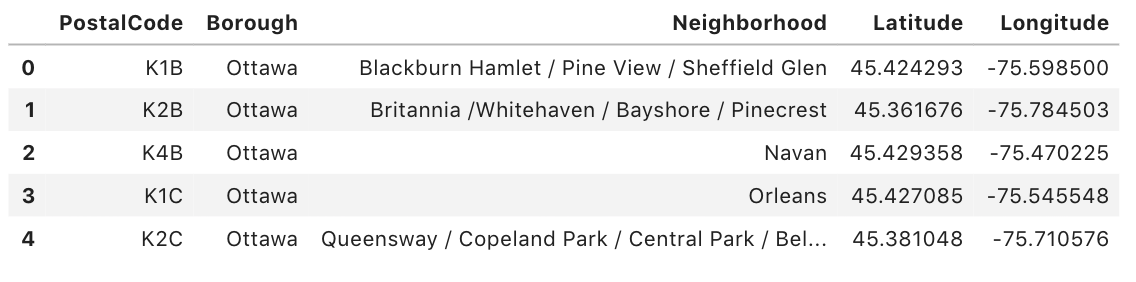
\includegraphics[width=1\columnwidth]{img/ottawa1.png}
        \caption{Sample of Ottawa neighborhoods.}
        \label{fig:ottawa_nei}
\end{figure}


\subsection{Data Feature}
To explore more information of Ottawa, using Foursquare api to explore the venues in each neighborhood of Ottawa. For each neighborhood, collecting the venue name and the venue category. The samples of collected data is shown in Fig. \ref{fig:ottawa_venue}.
\begin{figure}[]
        \centering
        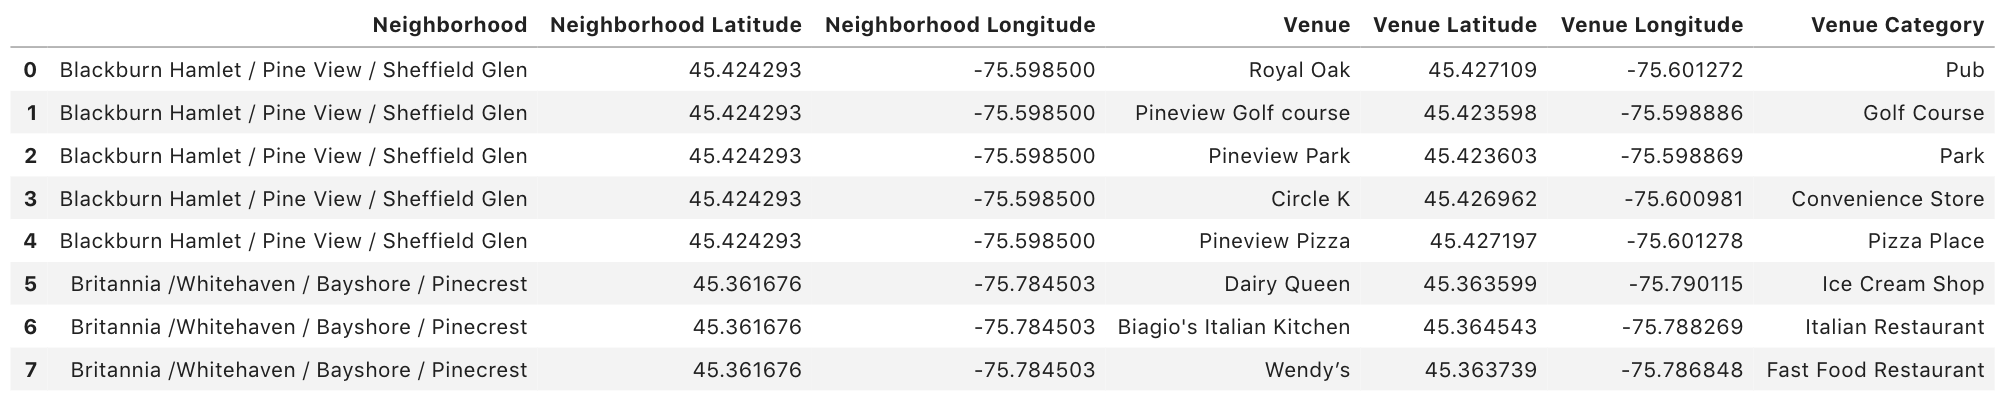
\includegraphics[width=1\columnwidth]{img/ottawa2.png}
        \caption{Sample of Ottawa venues.}
        \label{fig:ottawa_venue}
\end{figure}
\subsection{Data usage}
The collected data will be used in the following way: 
1. Explore the distribution of the restaurant and analyze the influence of the existing restaurants. 
2. Show the influence area of each restaurant. According to this information, we can choose the locations which are not covered by the current restaurant as candidates.
3. Cluster these restaurants and analyze the restaurant category of each cluster. Then, according to the ranked restaurant category, the best restaurant type in each cluster can be selected.


\section{CONCLUSION}
\label{sec:conclusion}
In this paper, we proposed RAU, a lightweight attention module designed to enhance the fine-grained feature extraction ability of standard CNN architectures. The proposed RAU can help the model effectively extract discriminative features. By adding RAU to two popular standard CNN architectures, we proposed two VMMR model, ResNet50-RAU and VGG16-RAU. We conducted a wide range of experiments on three benchmark VMMR datasets, including the evaluation under different environmental conditions. The experimental results on these three challenging vehicle datasets demonstrate our models surpass the traditional VMMR models and the state-of-the-art deep learning-based VMMR models. Especially, our models have stable performance under different environmental conditions. 

In addition, we proposed a one-stage VDFR model SSD-RAU to simultaneously detect and recognize the vehicle information. Our model achieves excellent fine-grained recognition performance and can be used in a real-time environment. We also conducted experiments on an object detection dataset, and the results demonstrate that SSD-RAU is also an excellent object detection model.




\bibliographystyle{IEEEtran}
\bibliography{Attention}




\end{document}